\chapter{Quantum Entanglements, Part 1}

These notes follow Leonard Susskind's opening lecture on quantum entanglement, with curation by LazyingArt LLC. The lecture begins, characteristically, with a sermon about intuition. It then turns that sermon into a program: we will not begin with wave mechanics, but with information, bits, configurations, update rules, and only then the elementary algebra that makes those update rules precise. The chapter should therefore be read in that order. We are being taught not merely a list of facts, but a way of rebuilding intuition.

\section{Why Quantum Mechanics Feels Unnatural}

Susskind begins by reminding us that our ordinary physical intuition is an evolutionary inheritance. It was formed in a world of rocks, arrows, prey, predators, and moderate velocities. Even an animal chasing another animal is already solving a problem in kinematics: it tracks relative velocity, direction, and the moment at which the sign of that relative velocity changes. So one should not underestimate how much classical mechanics is already wired into ordinary behavior.

But modern physics begins precisely where that inheritance stops being reliable. Relativity concerns velocities that no human or animal ever encountered in ordinary life. Quantum mechanics concerns electrons, uncertainty, and the breakdown of the very trajectory-based picture that ordinary experience encourages us to adopt. A particle, according to common sense, is a thing that has a position at every instant; if it has a position at every instant, then it has a trajectory; if it has a trajectory, then we compute its velocity from the differences of positions. That whole chain of intuition comes from the world of thrown stones and flying arrows. It is not a guide to the microscopic world.

So the problem is not that quantum mechanics is illogical. The problem is that it lies outside the regime that trained our brains. We therefore need abstraction before we can recover intuition. Susskind says, in effect, that physicists rewire themselves. They learn abstract mathematics first, and only afterward develop new habits of thought that make the subject feel less alien.

That sermon is not decorative. It explains the method of the lecture. This will not be a conventional first course in quantum mechanics, centered from the outset on the Schr\"odinger equation and the wave picture. The emphasis will be different. We are going to concentrate on the logic of quantum mechanics and the logic of quantum information. That is why the lecture pivots almost immediately to its first concrete object: the bit.

\section{Classical Bits and the Counting of States}

Physics, in this register, is information. To say something about a physical system is to provide information about it, often numerically, but very often in the form of a discrete alternative. Heads or tails, yes or no, up or down: these are all examples of the same logical structure.

\begin{definition}
A bit is a question about a system with exactly two possible answers.
\end{definition}

Susskind insists on starting with the classical case. A classical bit may be represented by \(0\) and \(1\), although the choice of symbols is arbitrary. We could equally well use \(1\) and \(-1\), or any other pair of labels. The point is only that there are two possibilities. Once that is fixed, we can write the two classical states as
\begin{equation}
|0\rangle,\qquad |1\rangle.
\end{equation}
At this stage the Dirac notation looks like excess baggage, and Susskind says so. It adds nothing to the classical description \emph{yet}. But it is installed here because it will be the natural notation later, when the bit becomes quantum.

For many bits we simply write a string inside the ket:
\begin{equation}
|001011\cdots\rangle.
\end{equation}
This is a configuration of a multibit system. The notation is intentionally plain. We are not yet taking tensor products apart; we are just recording a string of binary values.

Now comes the first quantitative question: how many states does such a system have? One bit has two states. Two bits have four. Each new bit doubles the number of possibilities. Therefore an \(n\)-bit classical system has
\begin{equation}
N_s=2^n
\end{equation}
possible configurations, where \(N_s\) is the number of states. Inverting the relation gives
\begin{equation}
n=\log_2 N_s.
\end{equation}

This is the point where the lecture turns the word \emph{bit} from a label into a measure. The number of bits of information carried by a system is, by definition, the logarithm base two of the number of available states:
\begin{equation}
I=\log_2 N_s.
\end{equation}
For systems built from binary alternatives this reproduces an integer. But the definition is broader. A die has six states, so its information content is \(\log_2 6\), which is not an integer. The definition survives even when the system is not literally built from a set of binary switches.

This is a small but important beat in the lecture. Susskind first defines the bit operationally, then counts states, then inverts the relation. The movement is deliberate: we are being taught to think of a state space as something whose size already measures information.

\section{How Ordinary Physics Becomes a Bit String}

The next question is the natural one: are bits merely a convenient language for toy systems such as coins, or do they really reach ordinary physics? Susskind's answer is emphatic. Almost any physical information can be represented by bits, at least approximately and often to arbitrarily improving approximation.

Begin with a single measured quantity, such as the temperature of a room. If we care only about finite accuracy, then we may truncate the value and write it in base two. Once that is done, the number is simply a finite string of zeros and ones. If we want more accuracy, we keep more places. If we want a finer notion of temperature, we redefine the unit and again represent the result in binary. The essential move is the same every time: finite accuracy turns a real-valued quantity into a long but finite bit string.

The same idea applies to fields. A field is something that varies from place to place. To encode it, we divide space into many small cells, order the cells, and record the field value in each cell with some chosen precision. The result is a long sequence of binary strings, one block per cell, and therefore a long sequence of bits. In that sense, a temperature field, an electric field, or a magnetic field may all be represented by binary data once we agree to discretize space and tolerate finite precision.

Susskind then gives a second example, even more directly in the language of yes-or-no questions. Impose a lattice on a room and suppose that no cell can contain more than one particle. Then each cell carries one bit:
\begin{equation}
\text{occupied} \longleftrightarrow 1,
\qquad
\text{empty} \longleftrightarrow 0.
\end{equation}
A particle configuration is thus encoded by a string of occupancies. What does the string mean? It means exactly this: the first cell is occupied, the second is empty, the third is empty, the fourth is occupied, and so on. We have traded a spatial picture for a sequence of answers to yes-or-no questions.

This is one of the lecture's recurring motifs: \emph{so far no quantum mechanics}. Nothing quantum has entered yet. We are still talking about classical information, classical bits, and classical approximation schemes. But the point is already substantial. If physical information can be encoded by bit strings, then digital computation is not an accident. That is why computers can simulate physics at all.

There is, however, a caveat, and the lecture states it explicitly. Exact classical real numbers may require infinitely many bits. Rational numbers may repeat, irrational numbers certainly do not terminate, and long-time classical tracking may demand more and more precision. But that does not disturb the practical or conceptual point being made here. It only sharpens it: a computer works because finite approximation is often enough, and because physical descriptions can be improved systematically by using more bits and finer discretization.

\section{Configurations, Update Rules, and State Space}

Up to this point the lecture has concentrated on how to \emph{describe} a system at one time. The next pivot is from description to law. A physical theory is not only a list of possible configurations; it must also tell us how one configuration becomes another.

\begin{definition}
A configuration is the state of a system at a given instant of time.
\end{definition}

Susskind is careful here. First comes configuration, not motion. We specify the state at one instant. Then, if we wish, we may discretize time as well as space and speak of updating from one digital instant to the next. In that language a physical theory consists of two parts: a space of possible states and a rule that updates one state into another slightly later state.

To make this visible, the lecture introduces an abstract state space. Its points are not points in ordinary space; they are entire configurations. That distinction matters. A closed loop in this state space is not a particle running around a spatial circle. It is a system moving through a cycle of possible configurations.

For a one-bit system the state space has only two points. Then the simplest possible update laws can be written in bare form:
\begin{equation}
0\mapsto 0,\qquad 1\mapsto 1,
\end{equation}
or
\begin{equation}
0\mapsto 1,\qquad 1\mapsto 0.
\end{equation}
The first is the trivial fixed-point law: nothing happens. The second is the flip-flop law: the system alternates forever between the two possibilities.

The same idea extends immediately to two bits. A two-bit system has four states. One perfectly good law moves the system around a closed loop in the logical space of those four configurations. Another good law describes two separate flip-flops happening in parallel. The lecture is not trying to exhaust the possibilities. It is trying to install a picture: the laws of motion may be drawn as arrows between states.

That is why the section matters. We are being led from a string of bits to a geometry of possibilities, and from there to dynamics as a pattern of arrows. Once that picture is in place, one further question becomes unavoidable: are all arrow patterns equally good?

\section{Reversibility, Information Loss, and Unitarity}

Now the lecture reaches its conceptual center. Susskind first shows examples of acceptable update laws, and then he draws another law that is logically easy to imagine but physically defective. Two distinct states flow into a single later state. Going forward is still defined. Going backward is not.

\begin{figure}[h]
\centering

\includegraphics[width=0.72\textwidth]{lecture_01_figure_02.png}
\caption{Board evidence from the discussion of reversible and irreversible update rules. The handwritten word \emph{unitarity} appears beside the emphasized four-state sketch.}
\end{figure}

\begin{figure}[h]
\centering
\resizebox{\linewidth}{!}{%
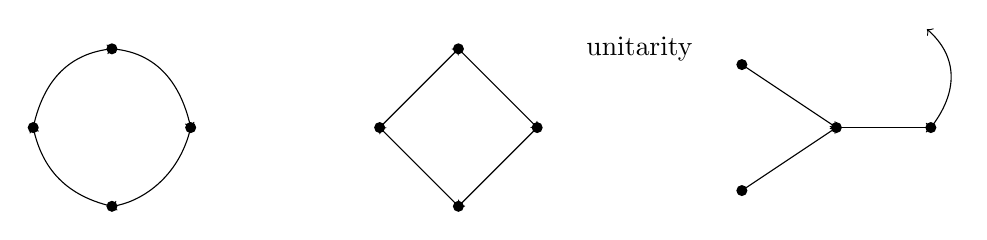
\begin{tikzpicture}[scale=1.0]
\fill (0,1) circle (2pt);
\fill (1,2) circle (2pt);
\fill (2,1) circle (2pt);
\fill (1,0) circle (2pt);
\draw[->] (0,1) .. controls (0.15,1.7) and (0.55,1.95) .. (1,2);
\draw[->] (1,2) .. controls (1.65,1.95) and (1.9,1.45) .. (2,1);
\draw[->] (2,1) .. controls (1.85,0.35) and (1.35,0.05) .. (1,0);
\draw[->] (1,0) .. controls (0.35,0.15) and (0.1,0.55) .. (0,1);

\fill (4.4,1) circle (2pt);
\fill (5.4,2) circle (2pt);
\fill (6.4,1) circle (2pt);
\fill (5.4,0) circle (2pt);
\draw[->] (4.4,1) -- (5.4,2);
\draw[->] (5.4,2) -- (6.4,1);
\draw[->] (6.4,1) -- (5.4,0);
\draw[->] (5.4,0) -- (4.4,1);
\node at (7.7,2) {unitarity};

\fill (9.0,1.8) circle (2pt);
\fill (9.0,0.2) circle (2pt);
\fill (10.2,1.0) circle (2pt);
\fill (11.4,1.0) circle (2pt);
\draw[->] (9.0,1.8) -- (10.2,1.0);
\draw[->] (9.0,0.2) -- (10.2,1.0);
\draw[->] (10.2,1.0) -- (11.4,1.0);
\draw[->] (11.4,1.0) .. controls (11.75,1.45) and (11.75,1.9) .. (11.35,2.25);
\end{tikzpicture}
}%
\caption{A clean schematic reconstruction of the board logic: reversible loops on the left, and a contrasting information-losing update rule on the right. The redraw stays schematic because the board does not securely label the states.}
\end{figure}

The good diagrams all have the same structural feature. Each state has one definite next state, but also one definite previous state. Susskind phrases this as the \emph{uniqueness of the future} and the \emph{uniqueness of the past}. That is what reversibility means here.

\subsection{Question \& Answer}

\paragraph{Question.} Why is the merging update rule forbidden? It seems perfectly sensible as a forward rule. If the system is here, it goes there. Why is that not enough?

\paragraph{Answer.} Because the rule destroys information about the past. If two distinct starting points both flow into the same later point, then once we arrive there we can no longer tell where we came from. The future is defined, but the past is not uniquely reconstructible. In Susskind's language, the rule loses information. At the fundamental level, where we imagine keeping track of every degree of freedom and not merely a coarse-grained summary, classical physics does not allow that.

This is the rhythm of the lecture: first a picture that looks reasonable, then the recognition that something has gone wrong, and then the sharpened principle that repairs it. The repair is not a matter of logic alone. Susskind explicitly says that such information-losing rules are logically conceivable; they are simply not the form taken by fundamental physical laws.

A second clarification follows immediately. Reversibility is not quite the same thing as exact time-reversal symmetry. A cyclic law still has an orientation: under forward evolution it runs one way around the loop, not both ways at once. What reversibility means is that there exists a reverse law taking us back uniquely. So the lecture draws a distinction between \emph{time reversibility} and the stronger notion of exact symmetry under interchange of past and future.

A third clarification comes from thermodynamics. It often \emph{looks} as if information is lost. Release the gas from one corner of a room and after a while the whole room looks the same no matter which corner we started from. But, Susskind argues, this is usually not fundamental loss. It is coarse-graining. We have stopped keeping track of the microscopic details. If we followed every molecule with enough precision, then in principle the information would still be there. What is lost in practice is our power to resolve it.

This is also the place where the lecture gestures beyond classical physics. Susskind jokes about naming the property ``unique-tarity,'' and then gives the quantum name: \emph{unitarity}. The quantum theory will have its own formal statement of this idea, but the principle has already appeared in classical dress: past and future must both be unique.

\section{Vectors, Rows, Columns, and Inner Products}

After the break Susskind says, in effect, that he was about to jump into quantum mechanics, but he wants to stop first and lay out some elementary mathematics. The timing matters. The algebra is not an isolated appendix; it is being installed because the classical discussion has made it necessary.

A vector is introduced in the least ceremonial possible way. Susskind does not begin with axioms of a vector space. He says plainly: a vector is a finite sequence of numbers. At this point the entries are real numbers. Complex conjugation, daggers, and the full quantum notation are postponed.

A four-component vector may be written as a row,
\begin{equation}
A=(A_1,A_2,A_3,A_4),
\end{equation}
or as a column,
\begin{equation}
A=
\begin{pmatrix}
A_1\\
A_2\\
A_3\\
A_4
\end{pmatrix}.
\end{equation}
The two forms contain the same information. They are simply different notations adapted to different operations. Susskind even warns us not to visualize these as arrows in ordinary space. For the present purpose they are just organized lists of numbers.

\begin{figure}[h]
\centering

\includegraphics[width=0.45\textwidth]{lecture_01_figure_03.png}
\caption{The board at the moment the lecture isolates a column vector. The entries are too small to transcribe literally, so the clean reconstruction uses generic components \(A_1,\dots,A_4\).}
\end{figure}

Now take a second vector, written as a row:
\begin{equation}
B=(B_1,B_2,B_3,B_4).
\end{equation}
If the row and the column have the same number of entries, we may multiply them. The rule is the familiar one:
\begin{equation}
BA=B_1A_1+B_2A_2+B_3A_3+B_4A_4.
\end{equation}
This is the inner product. It is not another vector. It is a single number. In ordinary three-dimensional language it would be called the dot product, and Susskind says so, but he prefers the more general name because the objects are being treated abstractly.

The pedagogical point is simple and operational. Rows multiply columns to produce scalars. Once that is secure, matrices can be introduced with almost no extra conceptual burden.

\section{Matrices as Update Operators}

A matrix is now presented as a machine that acts on a vector and produces a new vector. That description is intentionally concrete. We are not yet being handed the formal theory of linear operators. We are being given the piece of algebra that will encode update laws.

A \(4\times4\) matrix is written as
\begin{equation}
M=
\begin{pmatrix}
M_{11} & M_{12} & M_{13} & M_{14}\\
M_{21} & M_{22} & M_{23} & M_{24}\\
M_{31} & M_{32} & M_{33} & M_{34}\\
M_{41} & M_{42} & M_{43} & M_{44}
\end{pmatrix}.
\end{equation}
Its rows and columns are themselves collections of numbers, but together they define one operation. Acting on the column vector \(A\), the matrix produces a new column vector whose entries are row-by-column inner products:
\begin{equation}
(MA)_i=\sum_j M_{ij}A_j.
\end{equation}
Written out componentwise, the first two entries are
\begin{align}
(MA)_1 &= M_{11}A_1+M_{12}A_2+M_{13}A_3+M_{14}A_4,\\
(MA)_2 &= M_{21}A_1+M_{22}A_2+M_{23}A_3+M_{24}A_4.
\end{align}
The later entries are obtained in exactly the same way. Susskind does two and leaves the pattern to the audience.

\begin{figure}[h]
\centering

\includegraphics[width=0.82\textwidth]{lecture_01_figure_04.png}
\caption{Board layout for the discussion of a matrix acting on a column vector. The frame preserves the spatial organization of the explanation more reliably than the individual micro-entries.}
\end{figure}

\paragraph{A worked classical example.}
Now the lecture turns back to the classical discussion and shows why matrices matter. Suppose the system has finitely many configurations arranged in a cycle. Susskind first tries to draw a five-state example, then abandons it and retreats to four states so that the arithmetic will fit. That change does not alter the mathematical point.

We encode the four classical states by one-hot column vectors:
\begin{equation}
e_1=
\begin{pmatrix}
1\\0\\0\\0
\end{pmatrix},
\qquad
e_2=
\begin{pmatrix}
0\\1\\0\\0
\end{pmatrix},
\qquad
e_3=
\begin{pmatrix}
0\\0\\1\\0
\end{pmatrix},
\qquad
e_4=
\begin{pmatrix}
0\\0\\0\\1
\end{pmatrix}.
\end{equation}
The cycle \(1\to2\to3\to4\to1\) is represented by the permutation matrix
\begin{equation}
P=
\begin{pmatrix}
0&0&0&1\\
1&0&0&0\\
0&1&0&0\\
0&0&1&0
\end{pmatrix}.
\end{equation}
This is a deliberate clean convention. On the board the direction is corrected live, so the notes should not pretend that the first version written there was final. What is stable is the cyclic structure. With the present convention,
\begin{equation}
\begin{aligned}
Pe_1&=e_2,\qquad Pe_2=e_3,\\
Pe_3&=e_4,\qquad Pe_4=e_1.
\end{aligned}
\end{equation}
The same matrix acts on a general column by shifting its entries cyclically:
\begin{equation}
P
\begin{pmatrix}
A\\
B\\
C\\
D
\end{pmatrix}
=
\begin{pmatrix}
D\\
A\\
B\\
C
\end{pmatrix}.
\end{equation}
This is the lecture's first real worked example of an update rule written algebraically. A law of motion has become a matrix.

\paragraph{Matrix multiplication as repeated updating.}
Once a matrix represents one step of evolution, the reason for multiplying matrices by matrices becomes immediate. If
\begin{equation}
V'=MV,
\end{equation}
then a second step gives
\begin{equation}
V''=MV'=M^2V.
\end{equation}
So matrix multiplication composes updates. To evolve by two time steps, we apply the update matrix twice. To evolve by five, we multiply it into itself five times.

\begin{figure}[h]
\centering

\includegraphics[width=0.72\textwidth]{lecture_01_figure_05.png}
\caption{Board layout for the \(2\times2\) matrix product. The pedagogical point is that the right-hand matrix may be read column by column, each column being acted on by the left-hand matrix.}
\end{figure}

To make the arithmetic explicit, Susskind reduces the discussion to \(2\times2\) matrices:
\begin{equation}
M=
\begin{pmatrix}
M_{11} & M_{12}\\
M_{21} & M_{22}
\end{pmatrix},
\qquad
N=
\begin{pmatrix}
N_{11} & N_{12}\\
N_{21} & N_{22}
\end{pmatrix}.
\end{equation}
Their product \(C=MN\) is another matrix. The first entry is obtained by taking the first row of \(M\) and multiplying it by the first column of \(N\):
\begin{equation}
C_{11}=M_{11}N_{11}+M_{12}N_{21}.
\end{equation}
The next entry comes from the first row of \(M\) and the second column of \(N\):
\begin{equation}
C_{12}=M_{11}N_{12}+M_{12}N_{22}.
\end{equation}
The general rule is
\begin{equation}
C_{ij}=\sum_k M_{ik}N_{kj}.
\end{equation}

The board layout in the lecture is especially revealing here. The right-hand matrix is drawn almost as two neighboring columns, because that is how Susskind wants us to think of it. Multiply the left matrix by the first column and put the result in the first column of the answer; multiply the left matrix by the second column and put the result in the second column of the answer. Matrix multiplication is thus visibly the same operation as matrix-times-vector multiplication, performed column by column.

\paragraph{Row vectors multiplied by matrices.}
The final pattern is the one obtained by multiplying a row vector by a matrix. If
\begin{equation}
B=(B_1,B_2,B_3,B_4),
\end{equation}
then \(BM\) is another row vector, and its \(j\)-th entry is found by multiplying the original row \(B\) by the \(j\)-th column of \(M\):
\begin{equation}
(BM)_j=\sum_i B_iM_{ij}.
\end{equation}

This closes the elementary algebra of the lecture. A row times a column is a number. A matrix times a column is a column. A row times a matrix is a row. A matrix times a matrix is a matrix. Susskind ends by stressing that if we can do these manipulations fluently, then we already possess the basic mathematics that quantum mechanics will use over and over again.

Only at the end, in the questions, does the lecture phrase reversibility in matrix language. A reversible update should be represented by a matrix with an inverse. That is the algebraic shadow of the earlier physical statement that there must be a unique future and a unique past.

\section{Summary}

The first lecture does not yet present the new quantum rules. Instead it prepares the ground with unusual care. First we are told why abstraction is necessary: ordinary intuition is a classical inheritance, not a trustworthy guide to the microscopic world. Then the lecture reframes physics as information. From there it constructs classical bits, counts their states, and shows how surprisingly much of ordinary physics may be represented by long strings of binary data.

Only after that groundwork does the lecture turn from configuration to law. A physical system consists of possible states together with an update rule. Not every conceivable update rule is acceptable: fundamental laws must preserve the distinction between different pasts, which is why reversibility and uniqueness of past and future become central. The quantum name for the corresponding principle has already been previewed: unitarity.

Finally, after the break, the lecture installs the algebraic machinery required for the next step. Vectors, inner products, matrices, and matrix multiplication are not side remarks. They are the clean language of updating. So the lecture ends exactly where it should end: classical bits have been lifted into linear algebra, and the stage is set for qubits.
